% generated by scripts/pkl_to_latex.py
% source PKL : uscan_v1_L8_Ne6_t1_mode-uniform_nmin2_solver-gcg_sz0_restarts10_iter300_kmax4_tol1em09_U1to20_N20-d03a74da789e.pkl
% scan type  : uscan
% state      : gs
% requires   : \usepackage{pgfplots} \pgfplotsset{compat=1.18}
% colours match the matplotlib PDF (tab10 cycle)
\definecolor{gmeC0}{HTML}{1F77B4}
\definecolor{gmeC1}{HTML}{FF7F0E}
\definecolor{gmeC2}{HTML}{2CA02C}
\definecolor{gmeC3}{HTML}{D62728}
\definecolor{gmeC4}{HTML}{9467BD}
\definecolor{gmeC5}{HTML}{8C564B}
\definecolor{gmeC6}{HTML}{E377C2}
\definecolor{gmeC7}{HTML}{17BECF}

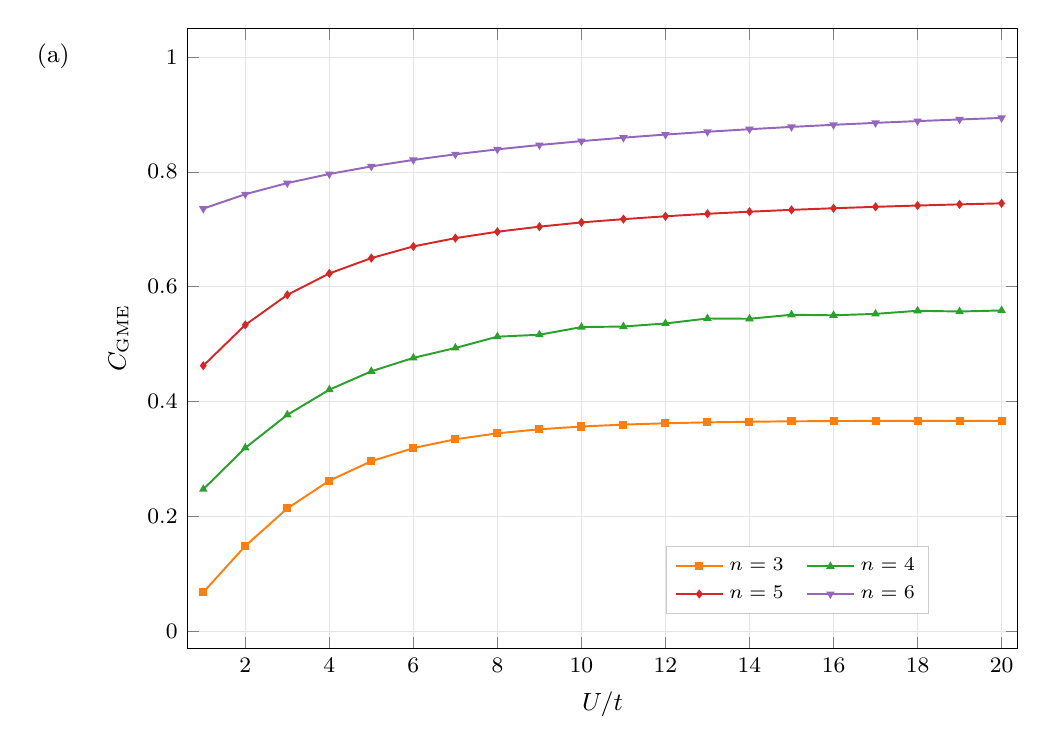
\begin{tikzpicture}
  \begin{axis}[
    width=\columnwidth,
    height=0.78\columnwidth,
    xlabel={$U/t$},
    ylabel={$C_{\mathrm{GME}}$},
    grid=both,
    grid style={line width=.1pt, draw=gray!20},
    tick label style={font=\footnotesize\rmfamily, /pgf/number format/fixed},
    label style={font=\small\rmfamily},
    scaled ticks=false,
    legend style={font=\scriptsize\rmfamily, draw=gray!40, at={(0.5,1.03)}, anchor=south, /tikz/every even column/.append style={column sep=6pt}},
    legend cell align={left},
    legend columns=2,
    ymin=-0.03,
    ymax=1.05,
    xmin=0.62,
    xmax=20.38,
    legend style={at={(0.735,0.110)}, anchor=center, fill=white},
    after end axis/.append code={\node[anchor=east, font=\small\rmfamily] at (axis description cs:-0.13,0.954) {(a)};},
  ]
    \addplot[color=gmeC1, mark=square*, mark size=1.1pt, line width=0.7pt] coordinates {
        (1,0.067809) (2,0.148367) (3,0.213758) (4,0.262161)
        (5,0.295938) (6,0.318826) (7,0.3342) (8,0.344557)
        (9,0.35159) (10,0.356408) (11,0.359732) (12,0.362033)
        (13,0.363623) (14,0.364711) (15,0.365441) (16,0.365913)
        (17,0.366196) (18,0.36634) (19,0.366383) (20,0.36635)
    };
    \addlegendentry{$n=3$}
    \addplot[color=gmeC2, mark=triangle*, mark size=1.1pt, line width=0.7pt] coordinates {
        (1,0.247133) (2,0.319239) (3,0.376745) (4,0.420513)
        (5,0.452539) (6,0.475918) (7,0.493151) (8,0.512852)
        (9,0.516191) (10,0.529536) (11,0.530541) (12,0.535825)
        (13,0.544502) (14,0.544023) (15,0.550995) (16,0.550077)
        (17,0.55255) (18,0.557932) (19,0.556703) (20,0.558466)
    };
    \addlegendentry{$n=4$}
    \addplot[color=gmeC3, mark=diamond*, mark size=1.1pt, line width=0.7pt] coordinates {
        (1,0.462285) (2,0.533404) (3,0.585638) (4,0.622958)
        (5,0.649689) (6,0.670001) (7,0.684432) (8,0.695583)
        (9,0.704422) (10,0.711817) (11,0.717516) (12,0.722498)
        (13,0.726854) (14,0.730501) (15,0.733686) (16,0.736492)
        (17,0.738985) (18,0.741214) (19,0.743221) (20,0.745038)
    };
    \addlegendentry{$n=5$}
    \addplot[color=gmeC4, mark=triangle*, mark size=1.1pt, mark options={rotate=180}, line width=0.7pt] coordinates {
        (1,0.735798) (2,0.760881) (3,0.780355) (4,0.796137)
        (5,0.809345) (6,0.820641) (7,0.830445) (8,0.83904)
        (9,0.846632) (10,0.85338) (11,0.85941) (12,0.864824)
        (13,0.869707) (14,0.874129) (15,0.87815) (16,0.881819)
        (17,0.885179) (18,0.888266) (19,0.89111) (20,0.893738)
    };
    \addlegendentry{$n=6$}
  \end{axis}
\end{tikzpicture}
